% Generated by plsimcount.pffigure -- do not edit; regenerate instead.
% figure: A-tte-by-order -- Suzuki formulas of each order, r from: Commutator bound (2021)
% source: results/pf-thesis/results.json
% metric=t gatebase=ct merged
% seed=1 t=n template=simcount synth=pygridsynth
% git_commit=c237fe494a6c663dd73df63b2b3fbb5e397a506e git_dirty=False
% source_sha256=6e8b2641428f03f62fe1dfd44b32f3373e9b382199e065d6a7d7340c7875a117
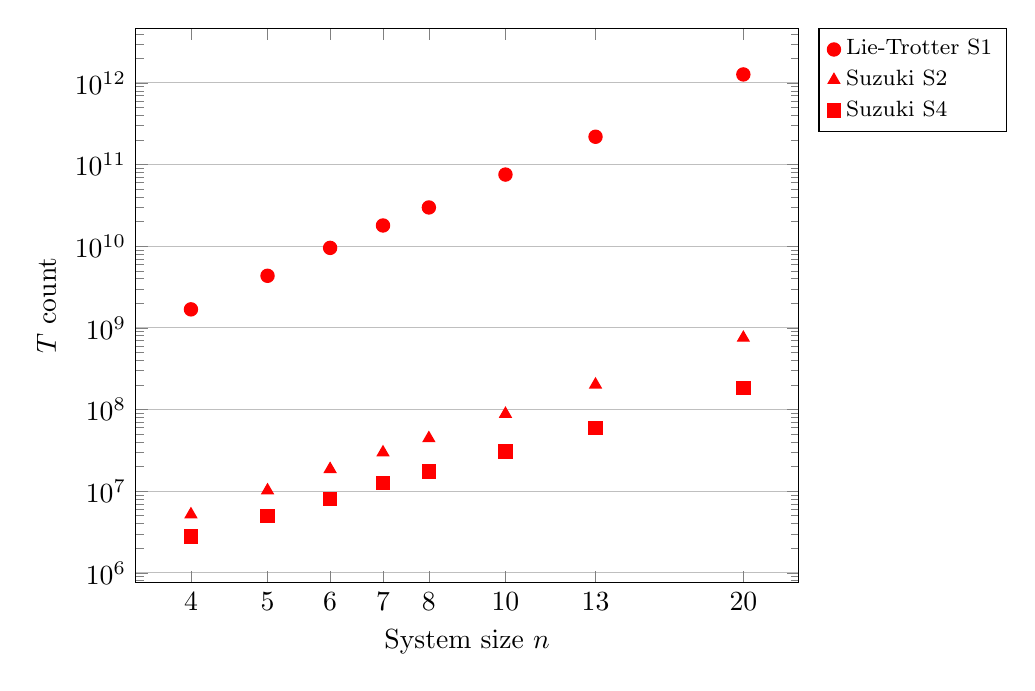
\begin{tikzpicture}
  \begin{loglogaxis}[
    width=10cm,
    xlabel={System size $n$},
    ylabel={$T$ count},
    xtick={4,5,6,7,8,10,13,20},
    xticklabels={4,5,6,7,8,10,13,20},
    ymajorgrids=true,
    legend pos=outer north east,
    legend cell align=left,
    legend style={font=\footnotesize},
  ]
    \addplot[only marks, red, mark=*, mark size=2.4pt, mark options={solid, fill=red}] coordinates {
      (4,1685202624)
      (5,4342683520)
      (6,9543017998)
      (7,17942187654)
      (8,29832119562)
      (10,75470365476)
      (13,219200151920)
      (20,1270851259104)
    };
    \addlegendentry{Lie-Trotter S1}
    \addplot[only marks, red, mark=triangle*, mark size=2.4pt, mark options={solid, fill=red}] coordinates {
      (4,5186260)
      (5,10202202)
      (6,18609080)
      (7,29759940)
      (8,44421936)
      (10,88321380)
      (13,201514950)
      (20,755181176)
    };
    \addlegendentry{Suzuki S2}
    \addplot[only marks, red, mark=square*, mark size=2.4pt, mark options={solid, fill=red}] coordinates {
      (4,2774736)
      (5,4948572)
      (6,8017436)
      (7,12608968)
      (8,17325630)
      (10,30462180)
      (13,59333200)
      (20,184135680)
    };
    \addlegendentry{Suzuki S4}
  \end{loglogaxis}
\end{tikzpicture}
